\documentclass[12pt]{article}
\usepackage[margin=1in]{geometry}
\usepackage{amsmath}
\usepackage{booktabs}
\usepackage{graphicx}
\usepackage{adjustbox}
\usepackage{listings}

\begin{document}
CS7347 HW3, Noah Gardner, 000843905\newline

\section{Assignment 3}
\begin{enumerate}
    % question 1
    \item Given the CFG grammar below. \textbf{[Points 30]}
          \newline
          \begin{tabular}{lll|l}
              \hline
              S  & $\rightarrow$ & NP VP       & 1.0 \\
              \hline
              VP & $\rightarrow$ & Vi          & 0.4 \\
              VP & $\rightarrow$ & Vt NP       & 0.4 \\
              VP & $\rightarrow$ & VP PP       & 0.2 \\
              \hline
              NP & $\rightarrow$ & DT NN       & 0.3 \\
              NP & $\rightarrow$ & NP PP       & 0.7 \\
              PP & $\rightarrow$ & IN NP       & 1.0 \\
              \hline
              Vi & $\rightarrow$ & 'sleeps'    & 1.0 \\
              Vt & $\rightarrow$ & 'saw'       & 1.0 \\
              NN & $\rightarrow$ & 'man'       & 0.7 \\
              NN & $\rightarrow$ & 'woman'     & 0.2 \\
              NN & $\rightarrow$ & 'telescope' & 0.1 \\
              DT & $\rightarrow$ & 'the'       & 1.0 \\
              IN & $\rightarrow$ & 'with'      & 0.5 \\
              IN & $\rightarrow$ & 'in'        & 0.5 \\
              \hline
          \end{tabular}
          \newline
          \begin{enumerate}
              \item Parse the sentence using the above grammar and show parse tree.
                    \textbf{[Points 10]}
                    \newline
                    \verb/The man saw the woman with the telescope./

                    \textbf{Answer:}
                    \begin{figure}[h]
                        \centering
                        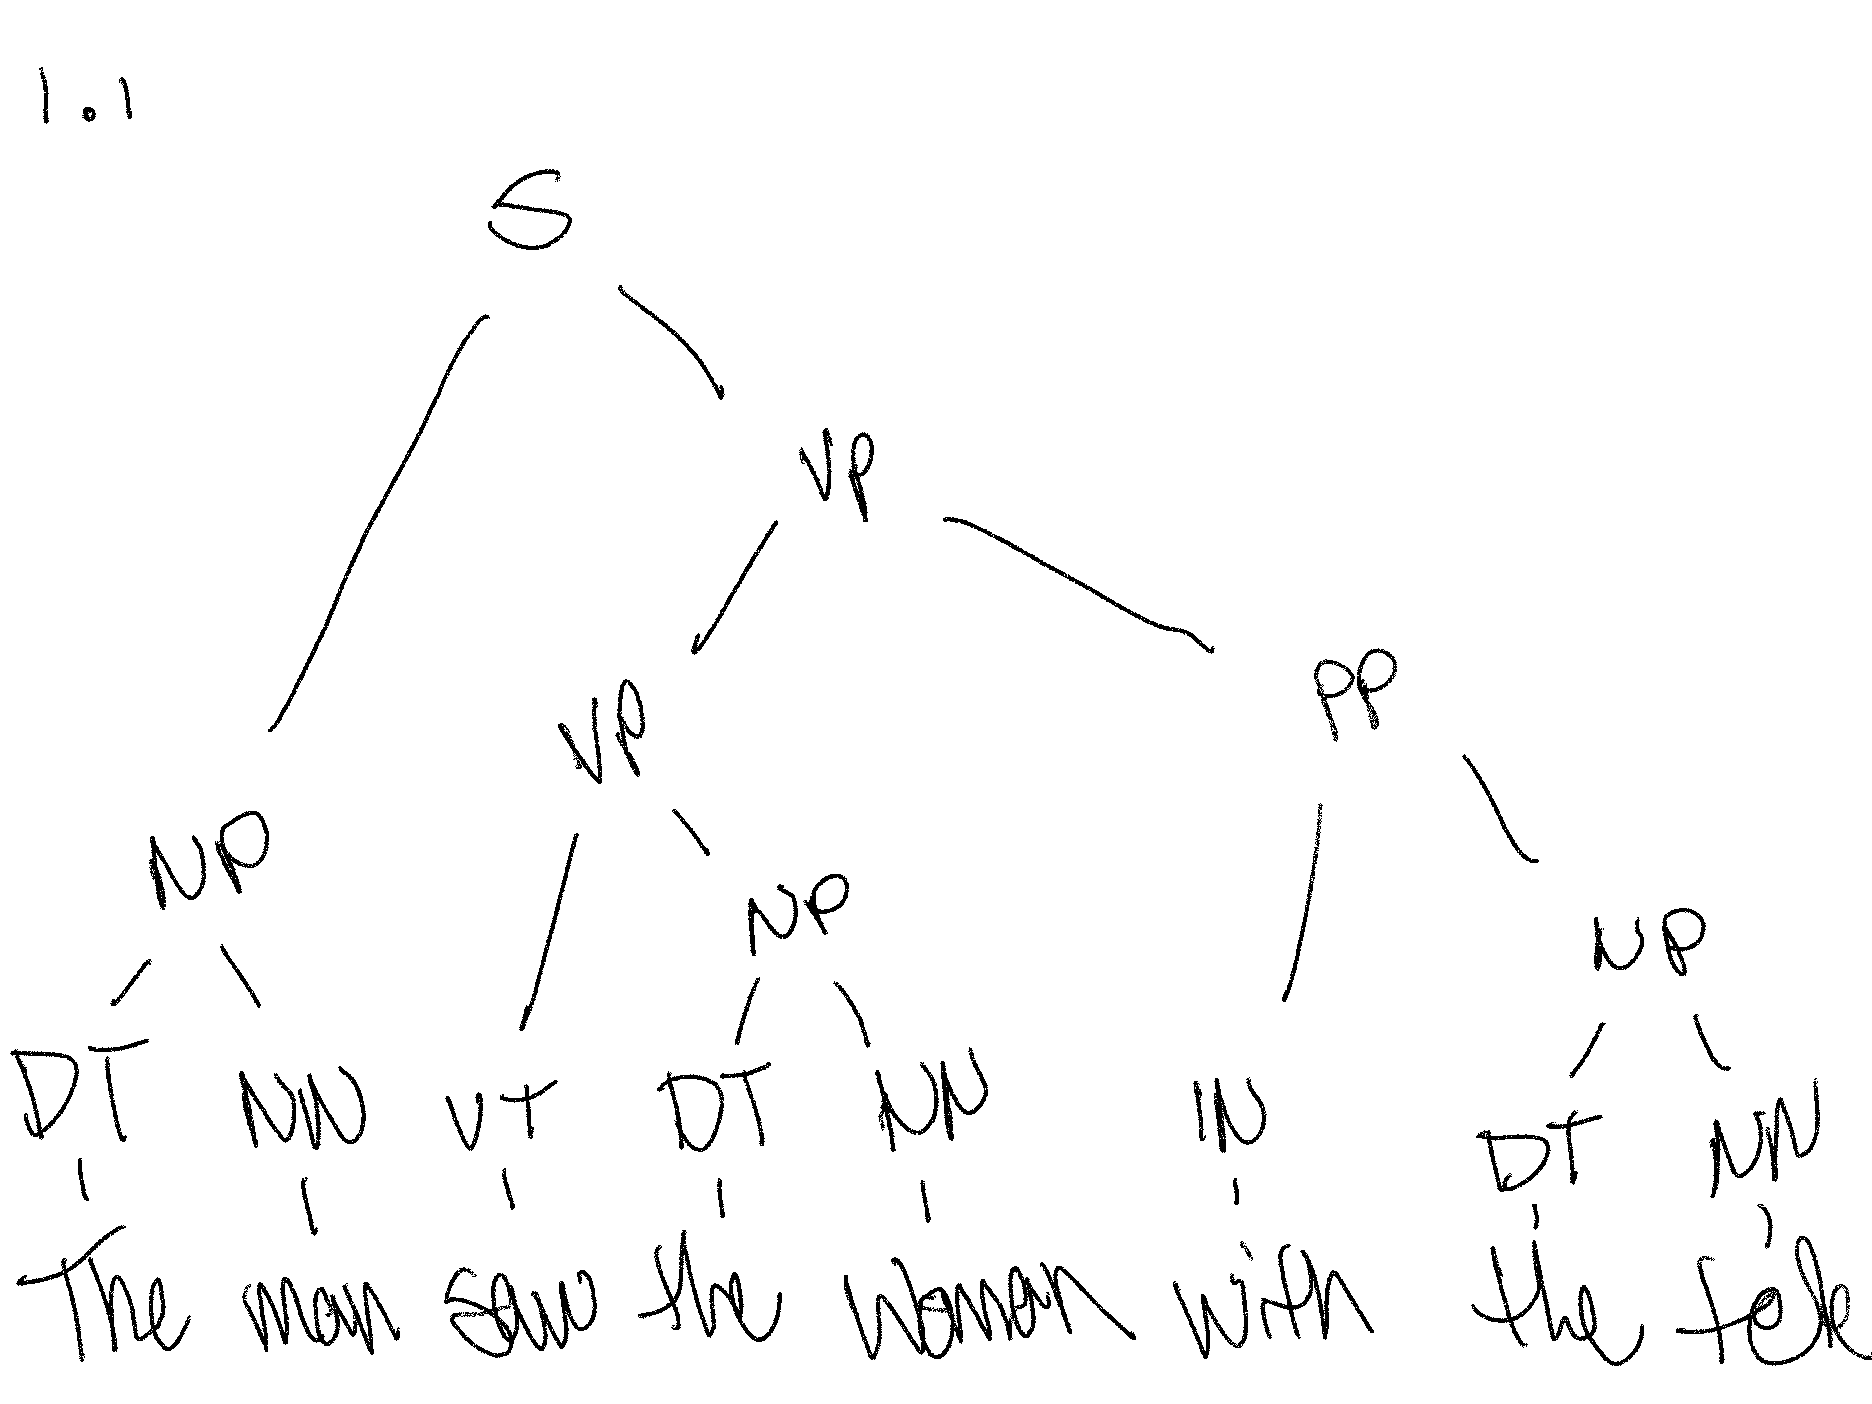
\includegraphics[width=0.7\textwidth]{assets/hw3/1_1.png}
                    \end{figure}
                    \newpage
              \item Show probabilisitc parse tree with probability at each
                    node in the tree for the following sentences.
                    \textbf{[Points 20]}
                    \newline
                    \verb/The man saw the woman with the telescope./

                    \textbf{Answer:}
                    \begin{figure}[h]
                        \centering
                        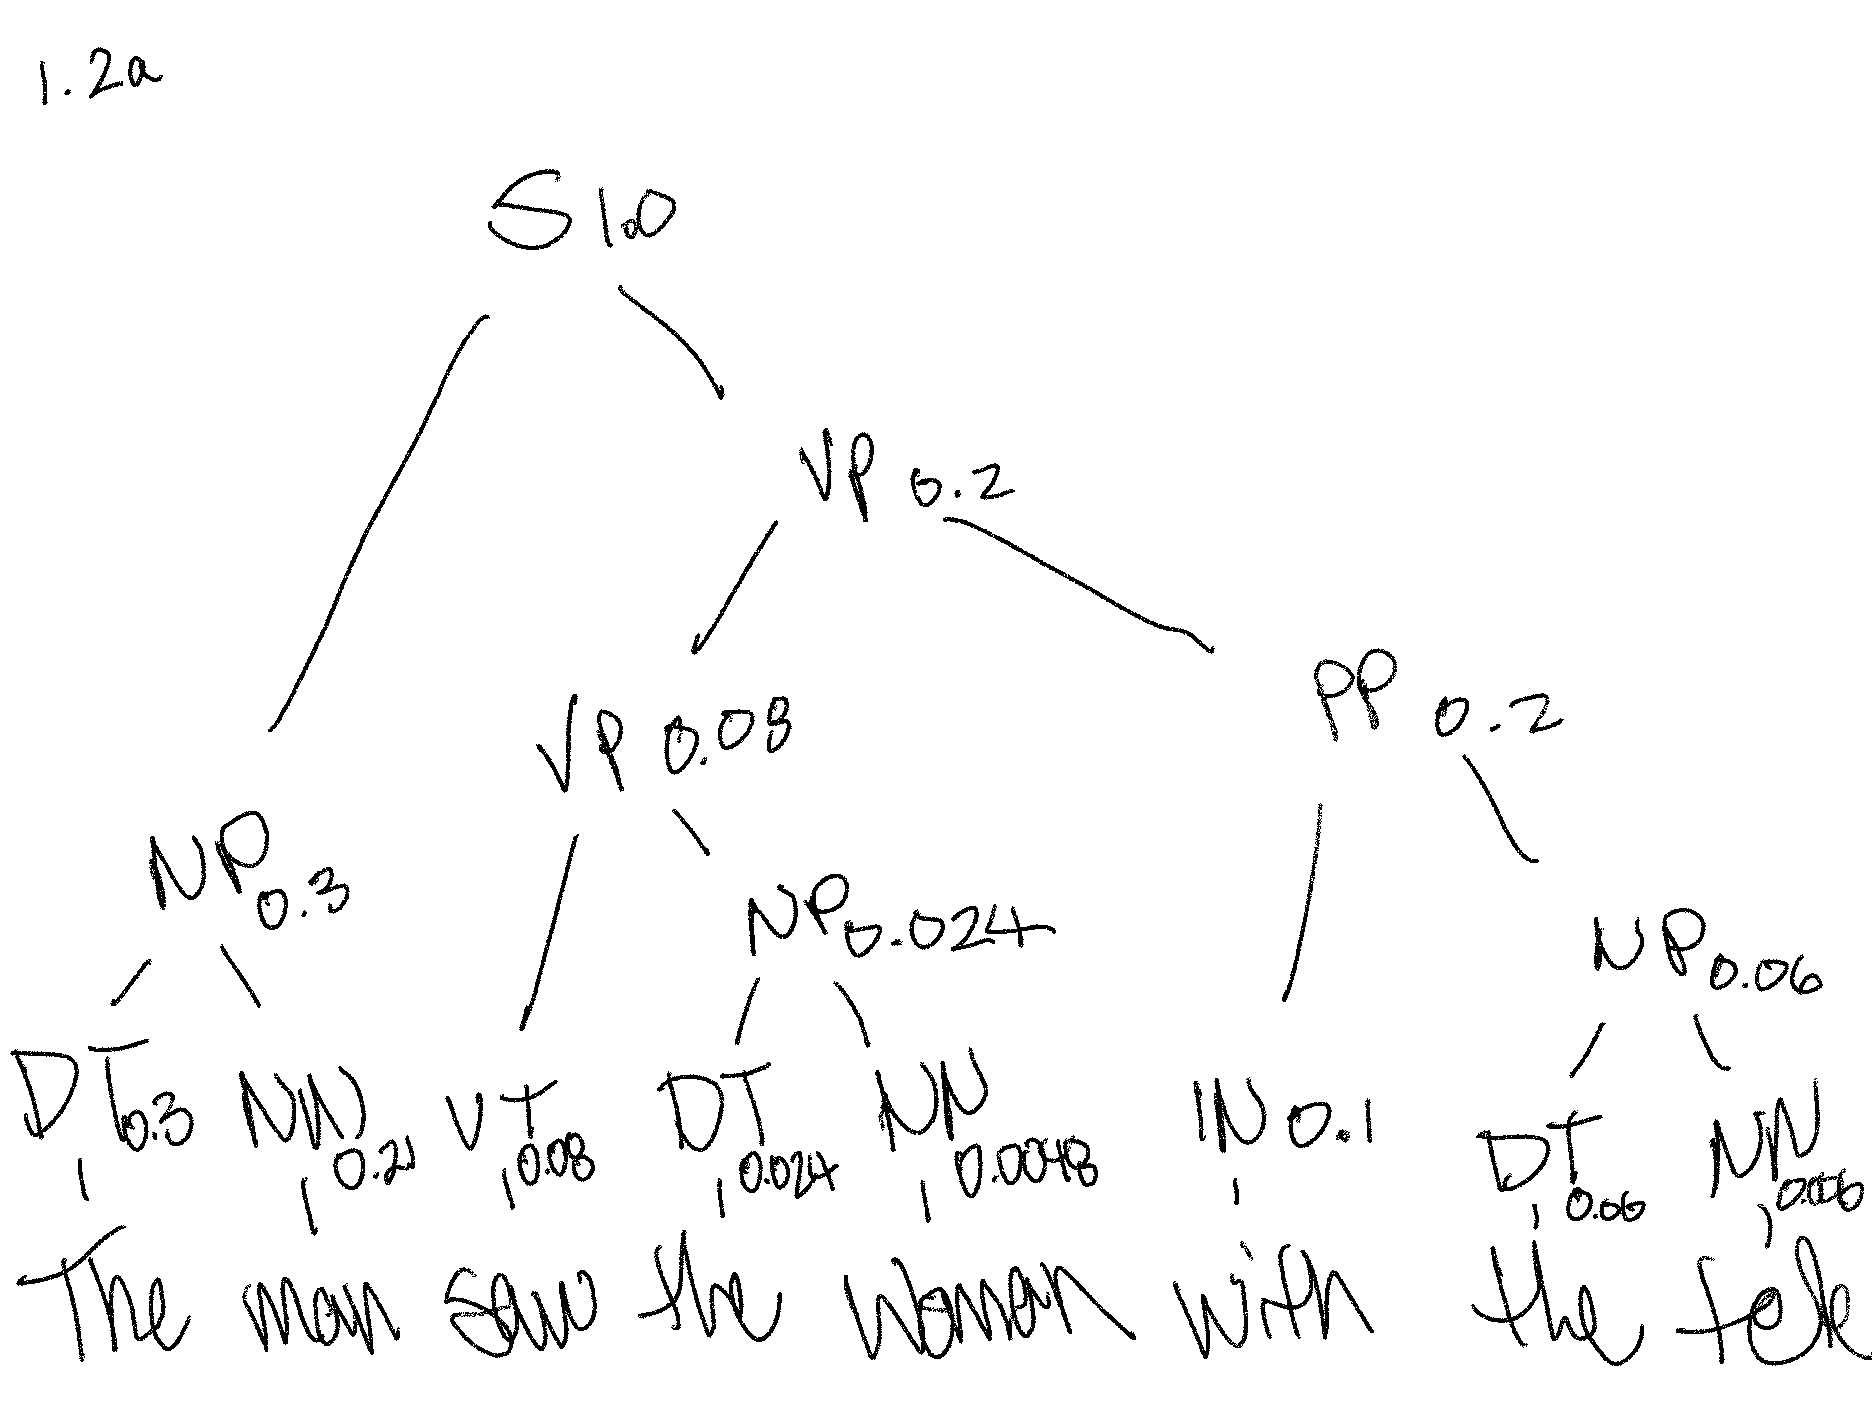
\includegraphics[width=0.65\textwidth]{assets/hw3/1_2a.png}
                    \end{figure}

                    \verb/The man sleeps./

                    \textbf{Answer:}
                    \begin{figure}[h]
                        \centering
                        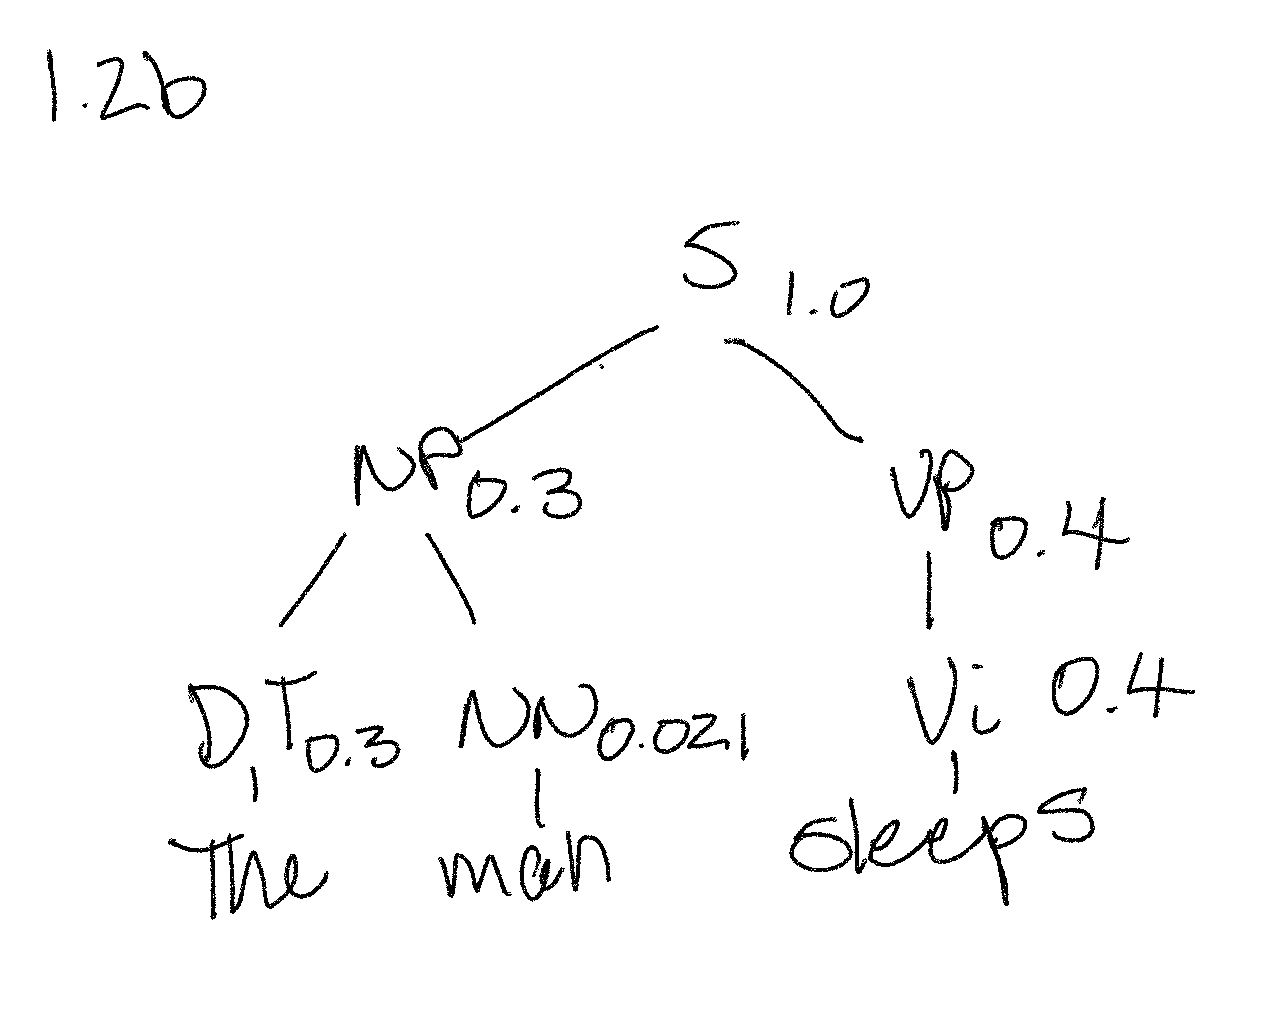
\includegraphics[width=0.65\textwidth]{assets/hw3/1_2b.png}
                    \end{figure}

          \end{enumerate}
          % question 2
          \newpage
    \item Show the bracketed notation for the following tree. \textbf{[Points 10]}
          \begin{figure}[h]
              \centering
              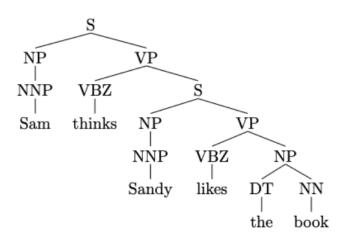
\includegraphics[width=0.5\textwidth]{assets/hw3/cfgtree.png}
          \end{figure}

          \textbf{Answer:}
          \begin{figure}[h]
              \centering
              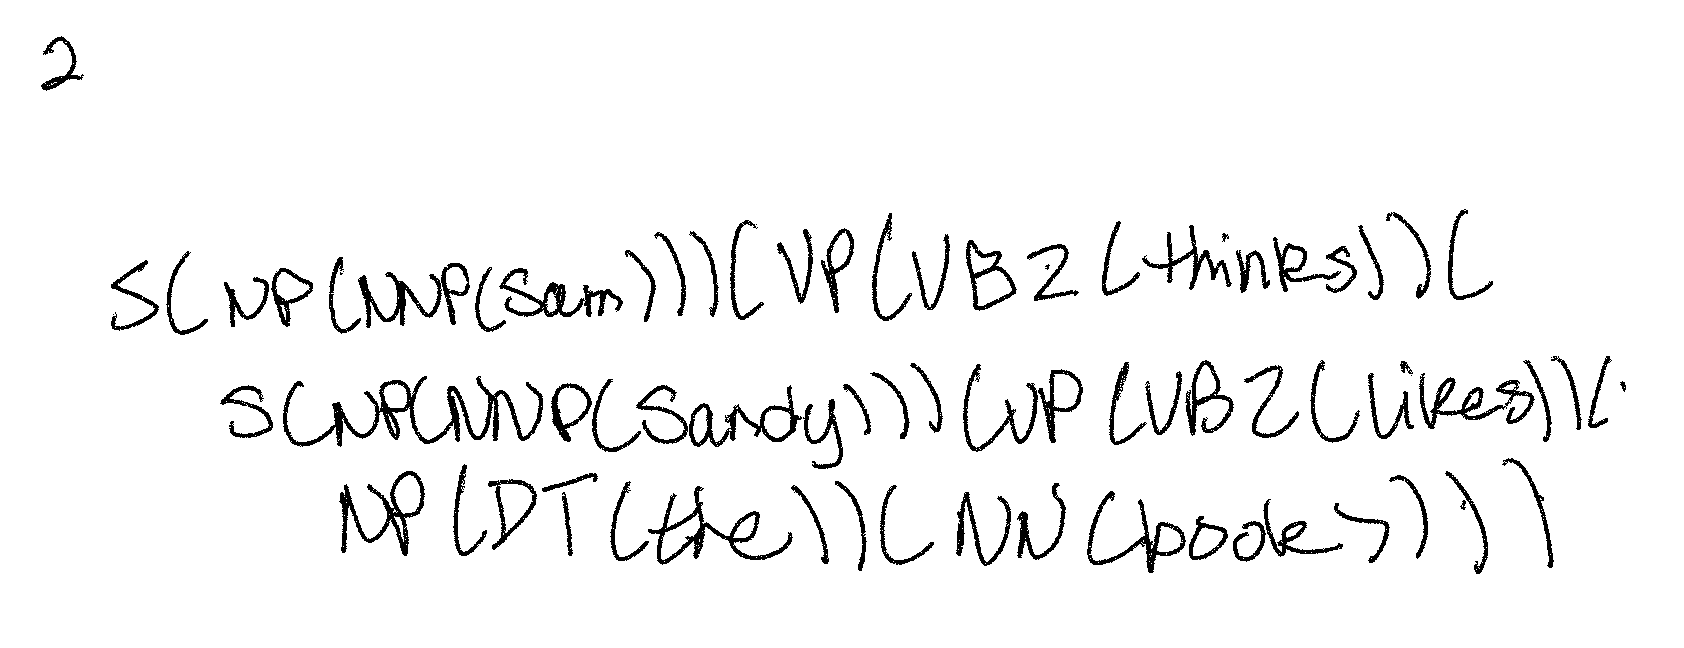
\includegraphics[width=0.65\textwidth]{assets/hw3/2.png}
          \end{figure}
          % question 3
          \newpage
    \item Consider the grammar G given by:
          \newline\newline
          \begin{tabular}{lll}
              S & $\rightarrow$ & XB      \\
              T & $\rightarrow$ & AB | XB \\
              X & $\rightarrow$ & AT      \\
              A & $\rightarrow$ & a       \\
              B & $\rightarrow$ & b       \\
          \end{tabular}
          \newline\newline
          Validate your answer by using CKY algorithm. \textbf{[Points 20]}
          \begin{enumerate}
              \item Is $w = aaabb$ in L(G)? \textbf{[Points 7.5]}

                    \textbf{Answer:}
                    \begin{figure}[h]
                        \centering
                        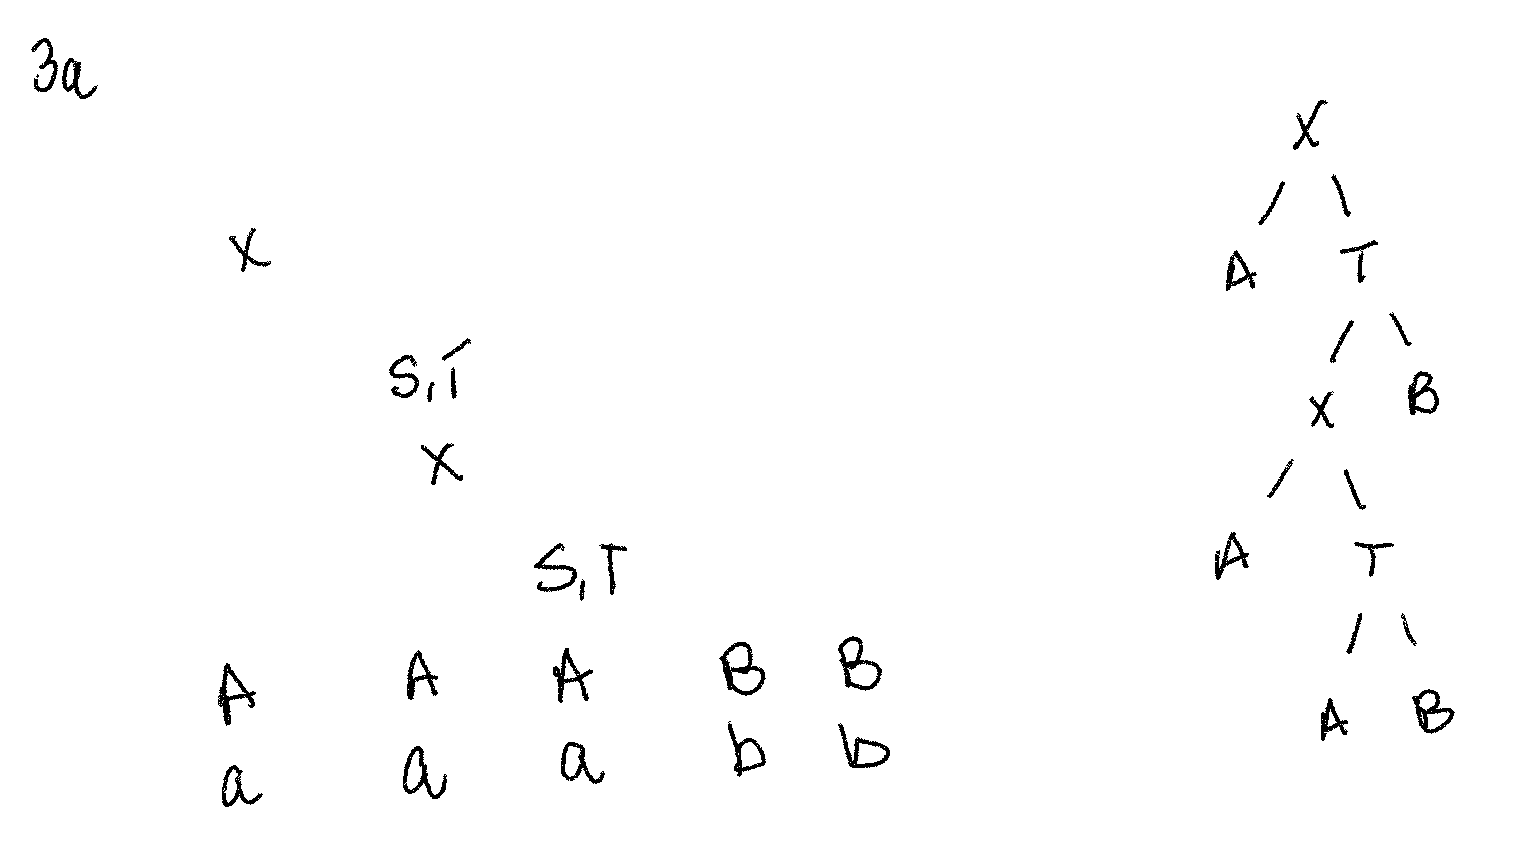
\includegraphics[width=0.65\textwidth]{assets/hw3/3a.png}
                    \end{figure}

              \item Is $w = aaabbb$ in L(G)? \textbf{[Points 7.5]}

                    \textbf{Answer:}
                    \begin{figure}[h]
                        \centering
                        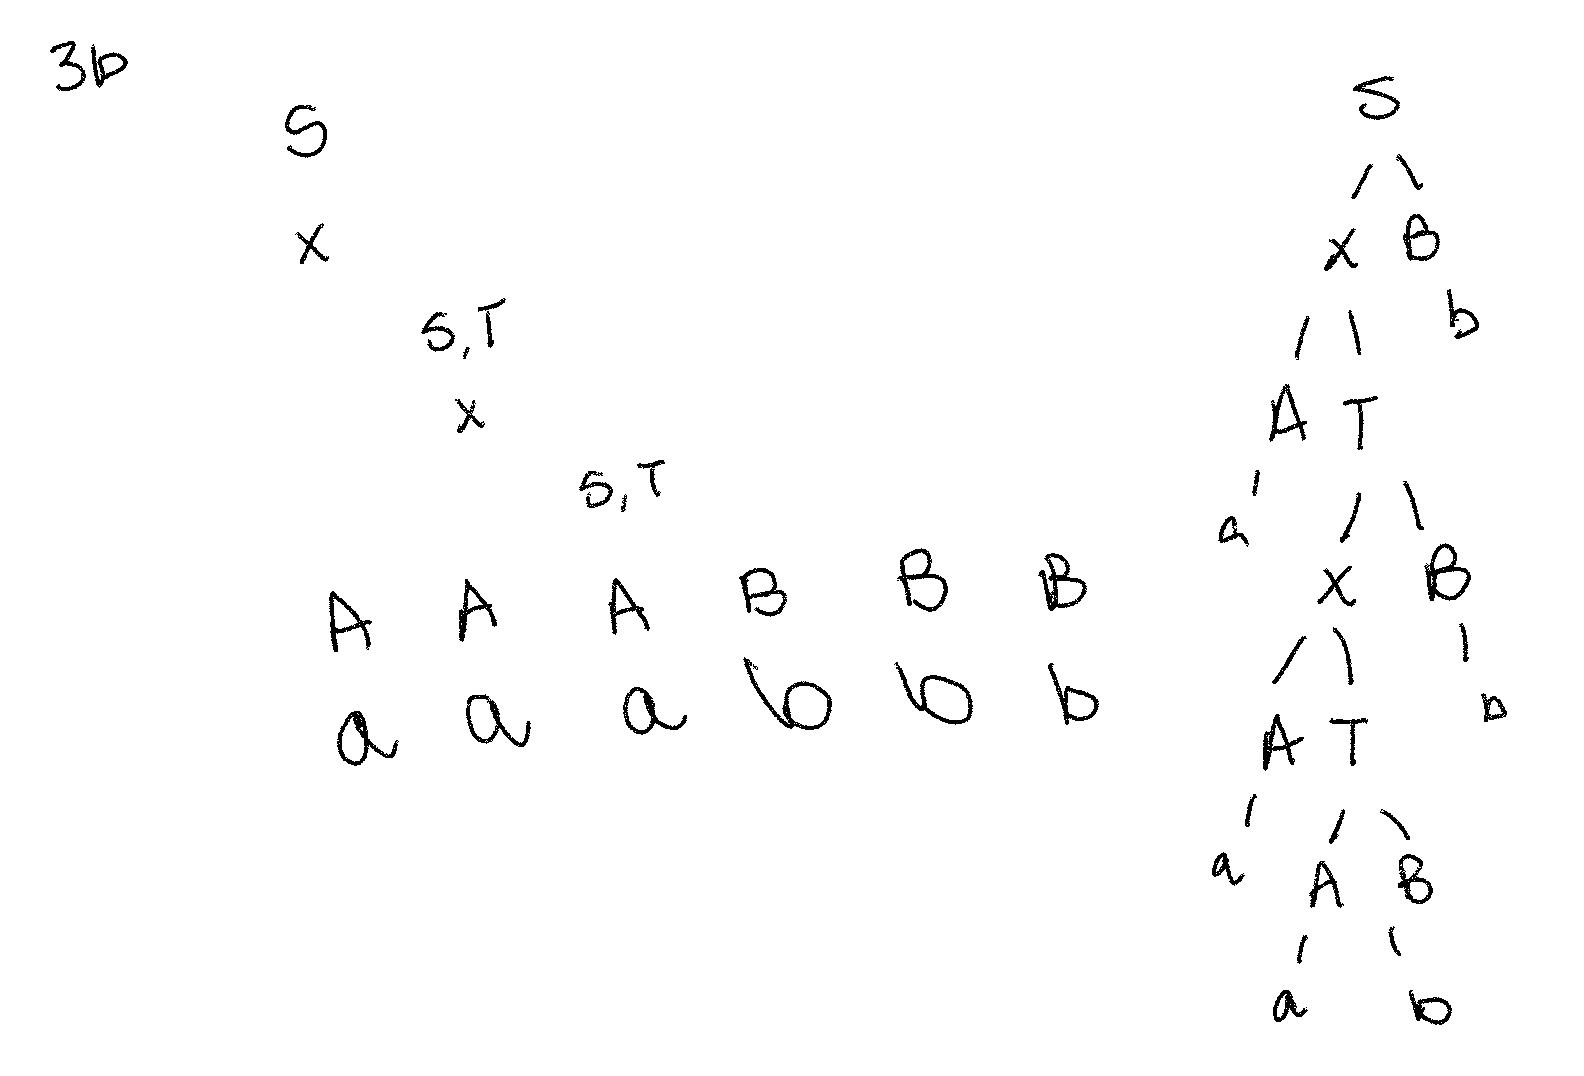
\includegraphics[width=0.65\textwidth]{assets/hw3/3b.png}
                    \end{figure}
          \end{enumerate}
          \newpage
          % question 4
    \item How are strings stored in spacy? Describe the document similarity checking
          mechanism in spacy? How would you compare similarity between two documents using spacy?
          Please write down an example code for document similarity checking. What are the spacy
          pipeline component initiated while using default nlp(). How would you add a custom component
          in the spacy nlp pipeline? Write a sample code which utilizes only two component tokenizer and
          add custom component in npl pipeline. \textbf{[Points 20]}

          \textbf{Answer:} Strings in spacy are stored as Documents. Document
          similarity uses a vector based model to compare two documents.

          Document similarity: \newline
          \begin{lstlisting}[language=python]
              import spacy

              nlp = spacy.load('en_core_web_md')
              d1 = nlp('document 1')
              d2 = nlp('document 2')
              print(d1.similarity(d2))
          \end{lstlisting}

          The default spacy pipeline components are tokenizer and parser. This
          is how to create a custom component. In this example, the custom
          component will delete extra tokens past 10.
          \begin{lstlisting}[language=python]
            import spacy
            from spacy.language import Language

            @Language.component('cutoff_component')
            def cutoff_component(doc):
                if len(doc) > 10:
                    return doc[:10]
                return doc

            nlp = spacy.load('en_core_web_sm')
            nlp.add_pipe(cutoff_component)
            doc = nlp('This is a sample document')
        \end{lstlisting}


          % question 5
    \item Go through the sequence of transitions needed for parsing the sentence:
          \newline
          \verb/I parsed this sentence correctly/.
          \newline
          The dependency tree is shown below. \textbf{[Points 25]}
          \begin{figure}[h]
              \centering
              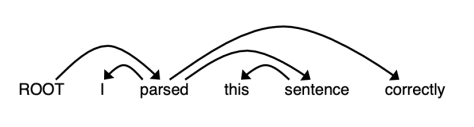
\includegraphics[width=0.5\textwidth]{assets/hw3/parsetree.png}
          \end{figure}
          \begin{enumerate}
              \item At each step, give the configuration of the stack and
                    buffer, as well as what transition was applied this step and what
                    new dependency was added (if any). \textbf{[Points 15]}

                    \textbf{Answer:} See table on next page.


              \item A sentence containing $n$ words will be parsed in how many
                    steps (in terms of n)? Briefly explain why.
                    \textbf{[Points 10]}

                    \textbf{Answer:} The sentence will be parsed in $2n$ steps,
                    because each word requires a step to push onto the stack,
                    and a step to pop from the stack.

          \end{enumerate}
\end{enumerate}

\rotatebox{90}{
    \begin{tabular}{l|l|l|l|c}
        Step & Stack                          & Buffer                                 & Transition       & Dependency                     \\
        0    & [root]                         & [I, parsed, this, sentence, correctly] & shift(I)         &                                \\
        1    & [root, I]                      & [parsed, this, sentence, correctly]    & shift(parsed)    &                                \\
        2    & [root, I, parsed]              & [this, sentence, correctly]            & leftarc          & parsed $\rightarrow$ I         \\
        3    & [root, parsed]                 & [this, sentence, correctly]            & shift(this)      &                                \\
        4    & [root, parsed, this]           & [sentence, correctly]                  & shift(sentence)  &                                \\
        5    & [root, parsed, this, sentence] & [correctly]                            & leftarc          & this $\leftarrow$ sentence     \\
        6    & [root, parsed, sentence]       & [correctly]                            & rightarc         & parsed $\rightarrow$ sentence  \\
        7    & [root, parsed]                 & []                                     & shift(correctly) &                                \\
        8    & [root, parsed, correctly]      & []                                     & rightarc         & parsed $\rightarrow$ correctly \\
        9    & [root, parsed]                 & []                                     & rightarc         & root $\rightarrow$ parsed      \\
    \end{tabular}
}
\end{document}
